\documentclass[runningheads]{llncs}
\usepackage[T1]{fontenc}
\usepackage{graphicx}
\graphicspath{{./images/}}
% Used for displaying a sample figure. If possible, figure files should
% be included in EPS format.
%
% If you use the hyperref package, please uncomment the following two lines
% to display URLs in blue roman font according to Springer's eBook style:
%\usepackage{color}
%\renewcommand\UrlFont{\color{blue}\rmfamily}
%
\begin{document}
% Just after the begin
%\begin{document}
\begin{titlepage}
\centering
{\bfseries\LARGE International University of Ecuador \ 
Faculty of Technical Sciences  \par}
\vspace{1cm}
{\scshape\Large School of Mecatronics engineering \par}
\vspace{3cm}
{\scshape\Huge Industrial Automatization \par}
\vspace{3cm}
{\itshape\Large Lab's report No 3: Timed relay applications \par}
\vfill
{\Large Author: \par}
{\Large Sebastian Osorio \par Pablo Guacho \par}
\vfill
{\Large Sep 2022 - Jan 2023 \par}
\end{titlepage}
\newpage


\title{Lab's report No 3\thanks{UIDE.}}
\author{Sebastian Osorio\inst{1}\orcidID{0000-0003-0106-5482} \and Pablo Guacho\inst{1}}

\authorrunning{S. Osorio. \& P. Guacho}

\institute{International University of Ecuador, Quito Av. Jorge Fernández and Av. Simón Bolívar 170201, Ecuador
    \email{seosoriogu@uide.edu.ec}
    \url{https://www.uide.edu.ec/} }

\maketitle

\textbf{Statement }Design  the  control  circuit  for  the  control  of  four  three-phase  motors,  which  work  under  the 
following condition:  
\begin{itemize}
    \item The motors are connected in star and the voltage applied to the motors is 380 V.here are four light signals H1, H2, H3 
    and H4 to indicate the operation of the motors. 
    \item The circuit will only have a start button S1 and an S0 for emergency stop. 
    \item H1, H2, H3 and H4 will be controlled by contactors K1, K2, K3 and K4 and their the operation is described in the
    figure~\ref{fig:sequence}. 
\end{itemize}

\begin{figure}[h]
    \centering
    \caption{Operation cycle}\label{fig:sequence}
    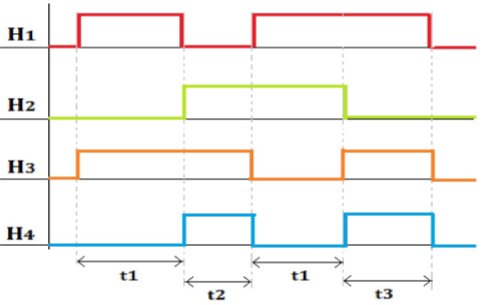
\includegraphics[scale = 0.75]{sequence.png}
\end{figure}

\section{Design}

It can be found in the following figure~\ref{fig:circuit} the design of the circuit. The circuit is designed to be able to represent the requested sequence.


\begin{figure}[h]
    \centering
    \caption{Circuit design}\label{fig:circuit}
    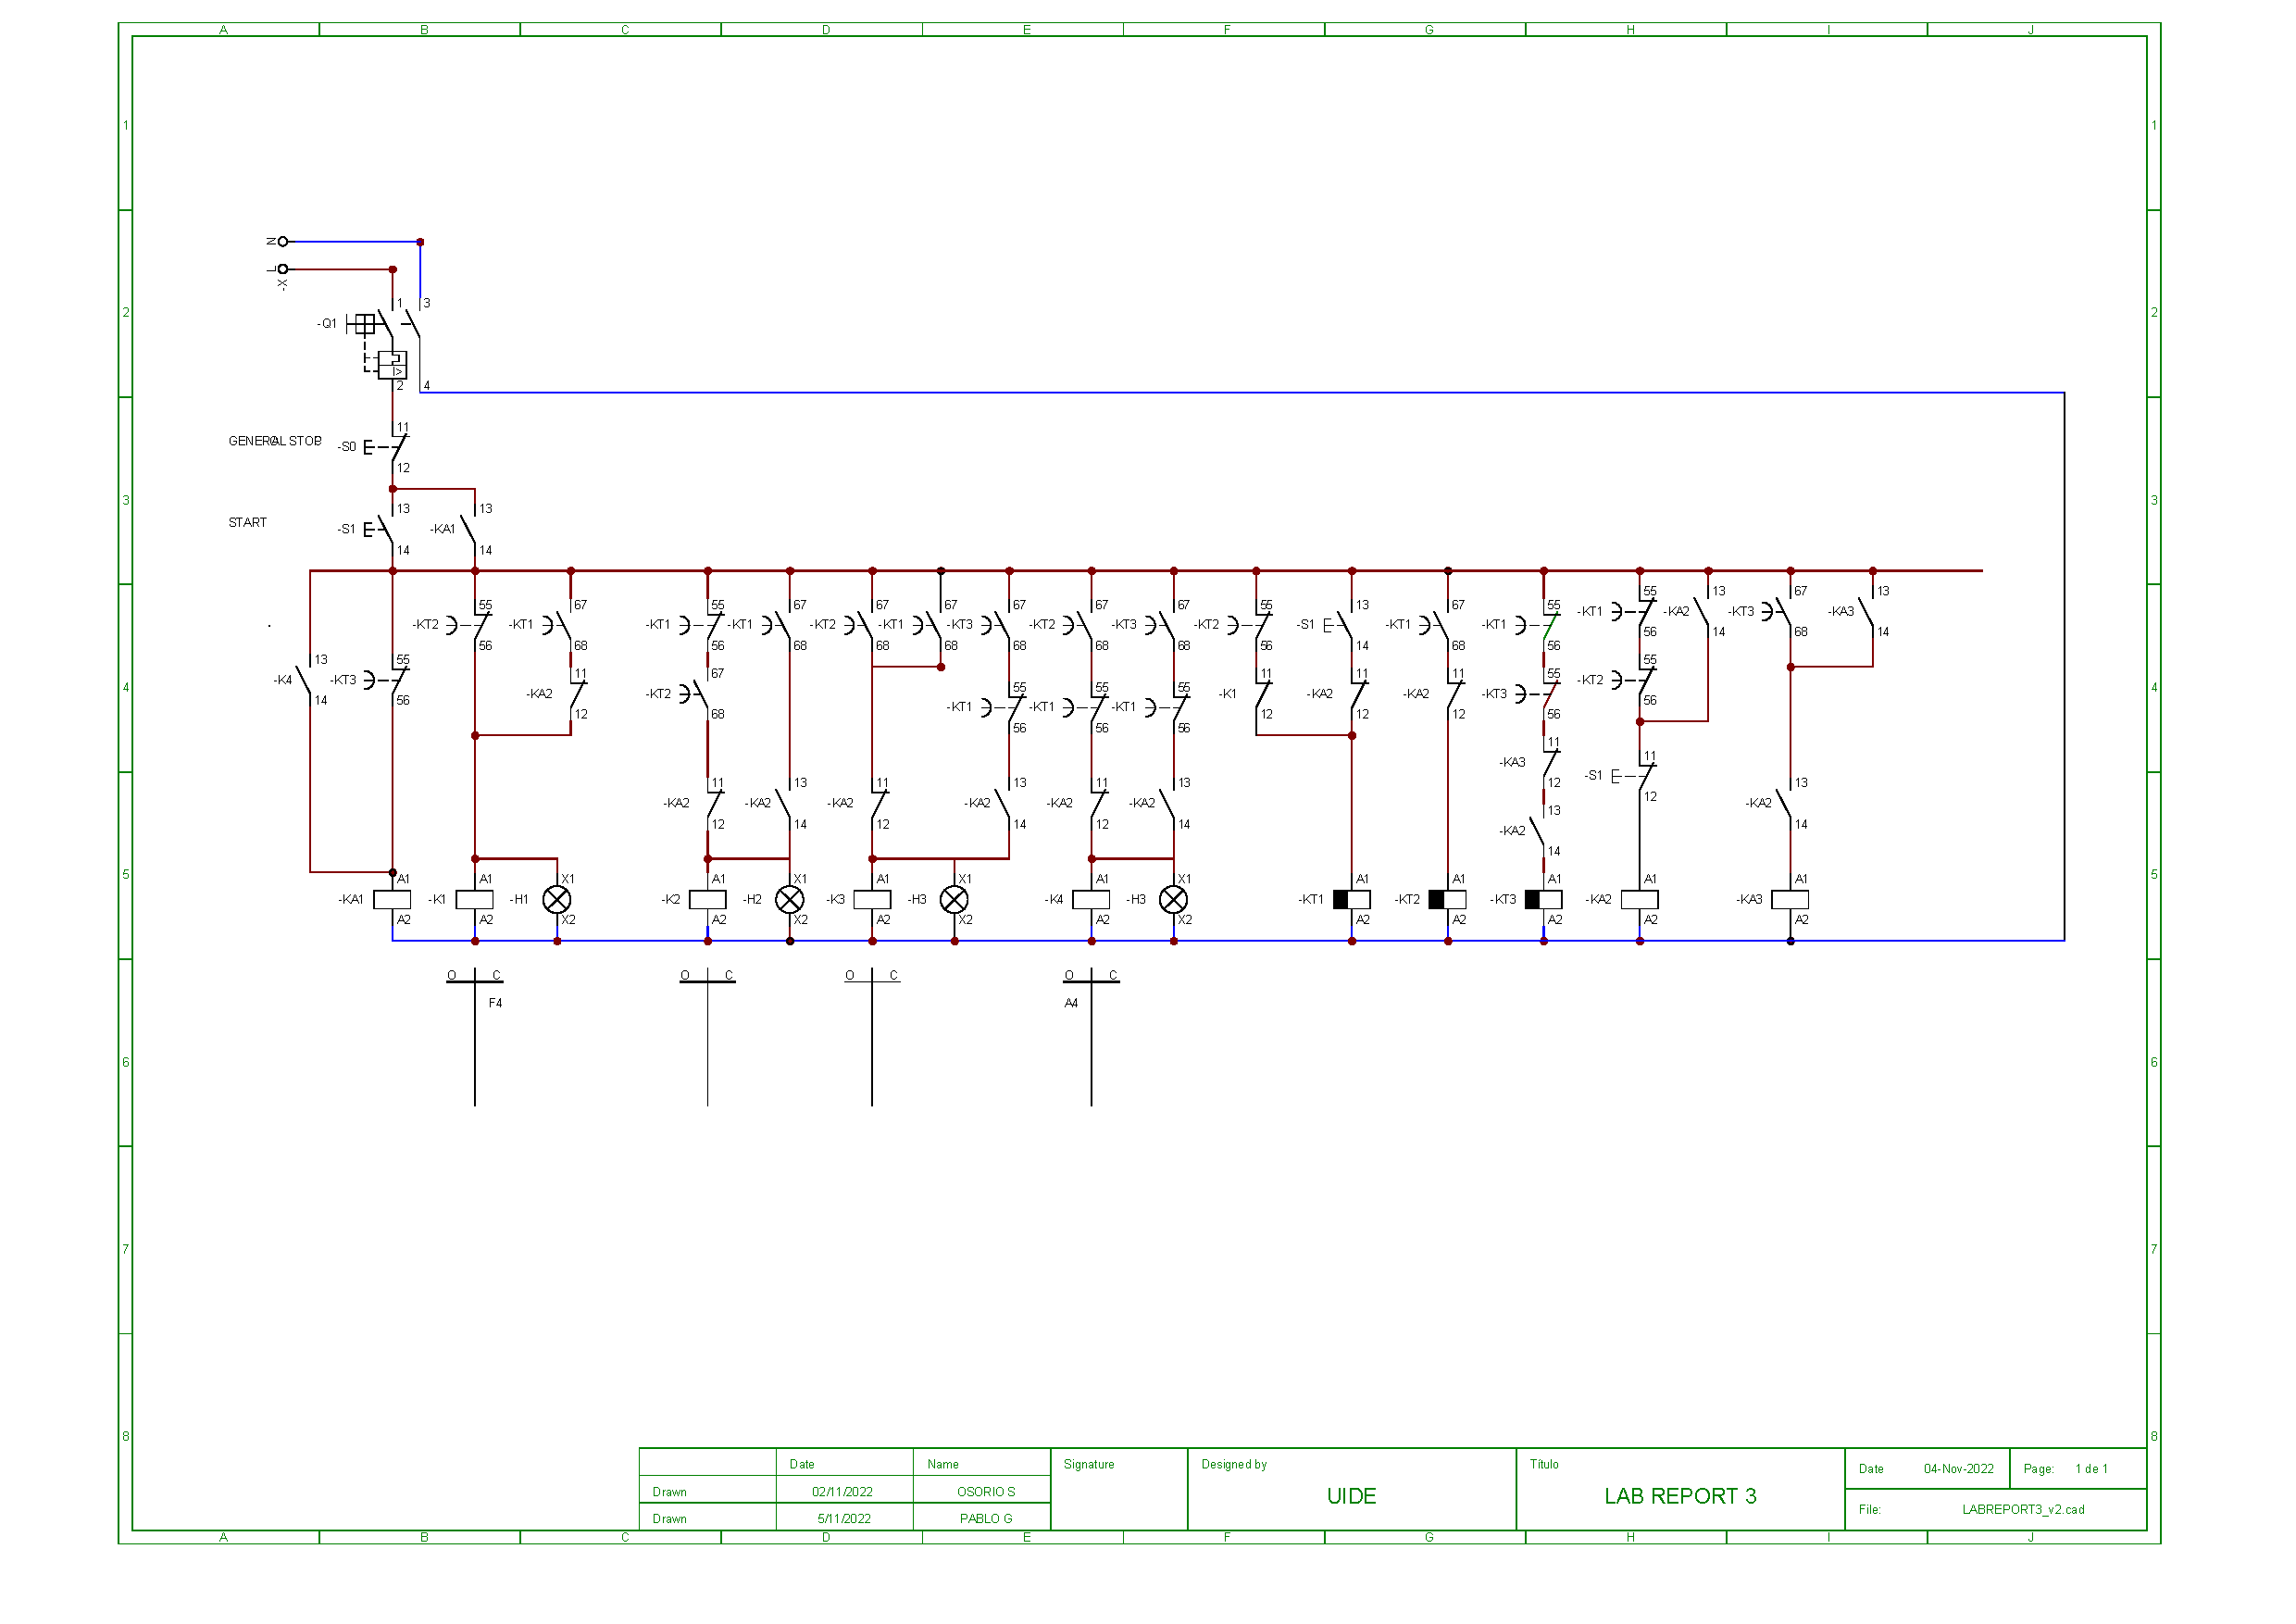
\includegraphics[width=\linewidth]{images/circuit.pdf}
\end{figure}


\section{Range of operation}

In this case the operation is not affected by the range of time t1>t2 or t1<t2. In fact it was design taking into account that all the times are the same such as  t1=t2=t3 


\section{Conclusion and recommendations}

The circuit was designed and tested with CADeSIMU. The circuit was tested to be able to follow the sequence of operation described in the figure~\ref{fig:sequence}. 
The circuit was tested with the following conditions for t1>t2 or t1<t2. It works in both cases. It is recommended to use the same time for all the times t1=t2=t3. However,
it present a little error at the end it shuts down immediately the timer t3 because if the off delay characteristics.


% \bibliographystyle{splncs04}
% \bibliography{mybibliography}
\end{document}